

\setkeys{Gin}{width=\textwidth}

%\subsection{Alternating Binomial Sums}
%% From ~/R/Pkgs/Rmpfr/inst/doc/Rmpfr-pkg.tex
%% or rather, the result of
%%    R CMD Rdconv --type=latex ~/R/Pkgs/Rmpfr/man/sumBinomMpfr.Rd
%%                            ---------------------------------------

\begin{frame}\frametitle{Alternating Binomial Sums}
Alternating binomial sums
appear in different contexts and are typically challenging,
i.e., currently impossible, to evaluate reliably as soon as $n$ is
larger than around $50 - 70$.

The alternating binomial sum $sB(f,n) :=$ \texttt{sumBinom(n, f, n0=0)} is
(up to sign) equal to the $n$-th forward difference operator $\Delta^n f$,
\begin{equation} \label{eq:sumBin}
 sB(f,n) := \sum_{k=0}^{n} (-1)^k {n \choose k}\cdot f(k) = (-1)^n \Delta^n f,
\end{equation}
where
\begin{equation}
  \label{eq:sumBin2}
  \Delta^n f = \sum_{k=0}^{n} (-1)^{n-k}{n \choose k}\cdot f(k)
\end{equation}
is the $n$-fold iterated forward difference
$\Delta f(x) = f(x+1) - f(x)$  (for $x = 0$).
\end{frame}

\begin{frame}[fragile]\frametitle{computing alternating binomial sums in R}
An obvious R implementation of
\(
 sB(f,n) = \sum_{k=0}^{n} (-1)^k {n \choose k}\cdot f(k)
\),
\medskip

\begin{Schunk}
\begin{Sinput}
> sumBinom <- function(n, f, n0=0, ...) {
+   k <- n0:n
+   sum( choose(n, k) * (-1)^k * f(k, ...))
+ }
> ## and the same for a whole *SET* of  n  values:
> sumBin.all.R <- function(n, f, n0=0, ...)
+    sapply(n, sumBinom, f=f, n0=n0, ...)
\end{Sinput}
\end{Schunk}
\bigskip

Will see: gets numerical problems, for relatively small $n$ even for well
behaved functions $f(\cdot)$.
\end{frame}

\begin{frame}[fragile]
The \texttt{Rmpfr} version is pretty simple, as well:

\medskip

\begin{Schunk}
\begin{Sinput}
> sumBinomMpfr
\end{Sinput}
\begin{Soutput}
function (n, f, n0 = 0, alternating = TRUE, precBits = 256) 
{
    stopifnot(0 <= n0, n0 <= n, is.function(f))
    sum(chooseMpfr.all(n, k0 = n0, alternating = alternating) * 
        f(mpfr(n0:n, precBits = precBits)))
}
<environment: namespace:Rmpfr>
\end{Soutput}
\end{Schunk}
\smallskip

and has a corresponding version for a full set of $n$:
\end{frame}

\begin{frame}[fragile]
Compute  \code{sumBinomMpfr(n)} for a whole set of 'n' values:
\begin{Schunk}
\begin{Sinput}
> sumBin.all <- function(n, f, n0=0, precBits = 256, ...)
+ {
+   N <- length(n)
+   precBits <- rep(precBits, length = N)
+   ll <- lapply(seq_len(N), function(i)
+            sumBinomMpfr(n[i], f, n0=n0, precBits=precBits[i], ...))
+   sapply(ll, as, "double")
+ }
\end{Sinput}
\end{Schunk}
\medskip
((Note that \code{sapply(.)} is not directly applicable, because its
 ``simplify'' part behaves wrongly with vectors of ``mpfr'' numbers.))
\end{frame}

\begin{frame}[fragile]\frametitle{Comparison ``double'' vs ``mpfr'':}
For comparison, computing the alternating binomial sum,
\begin{equation*}
 sB(f,n) := \sum_{k=0}^{n} (-1)^k {n \choose k}\cdot f(k),
\end{equation*}
now try the simple  $f(x) = \sqrt{x}$, i.e., in R, \texttt{sqrt(x)}:
\medskip

\begin{Schunk}
\begin{Sinput}
> nn <- 5:80
> system.time(res.R   <- sumBin.all.R(nn, f = sqrt)) ## instant!
\end{Sinput}
\begin{Soutput}
   user  system elapsed 
  0.002   0.000   0.002 
\end{Soutput}
\begin{Sinput}
> system.time(resMpfr <- sumBin.all  (nn, f = sqrt)) ## ~2 seconds
\end{Sinput}
\begin{Soutput}
   user  system elapsed 
  1.525   0.007   1.573 
\end{Soutput}
\end{Schunk}
\end{frame}

\begin{frame}[fragile]
\begin{Schunk}
\begin{Sinput}
> matplot(nn, cbind(res.R, resMpfr), type = "l", lty=1,
+         ylim = extendrange(resMpfr, f = 0.25), xlab = "n",
+         main = "sumBinomMpfr(n, f = sqrt)  vs.  R double precision")
> legend("topleft", leg=c("double prec.", "mpfr"), lty=1, col=1:2, bty = "n")
\end{Sinput}
\end{Schunk}
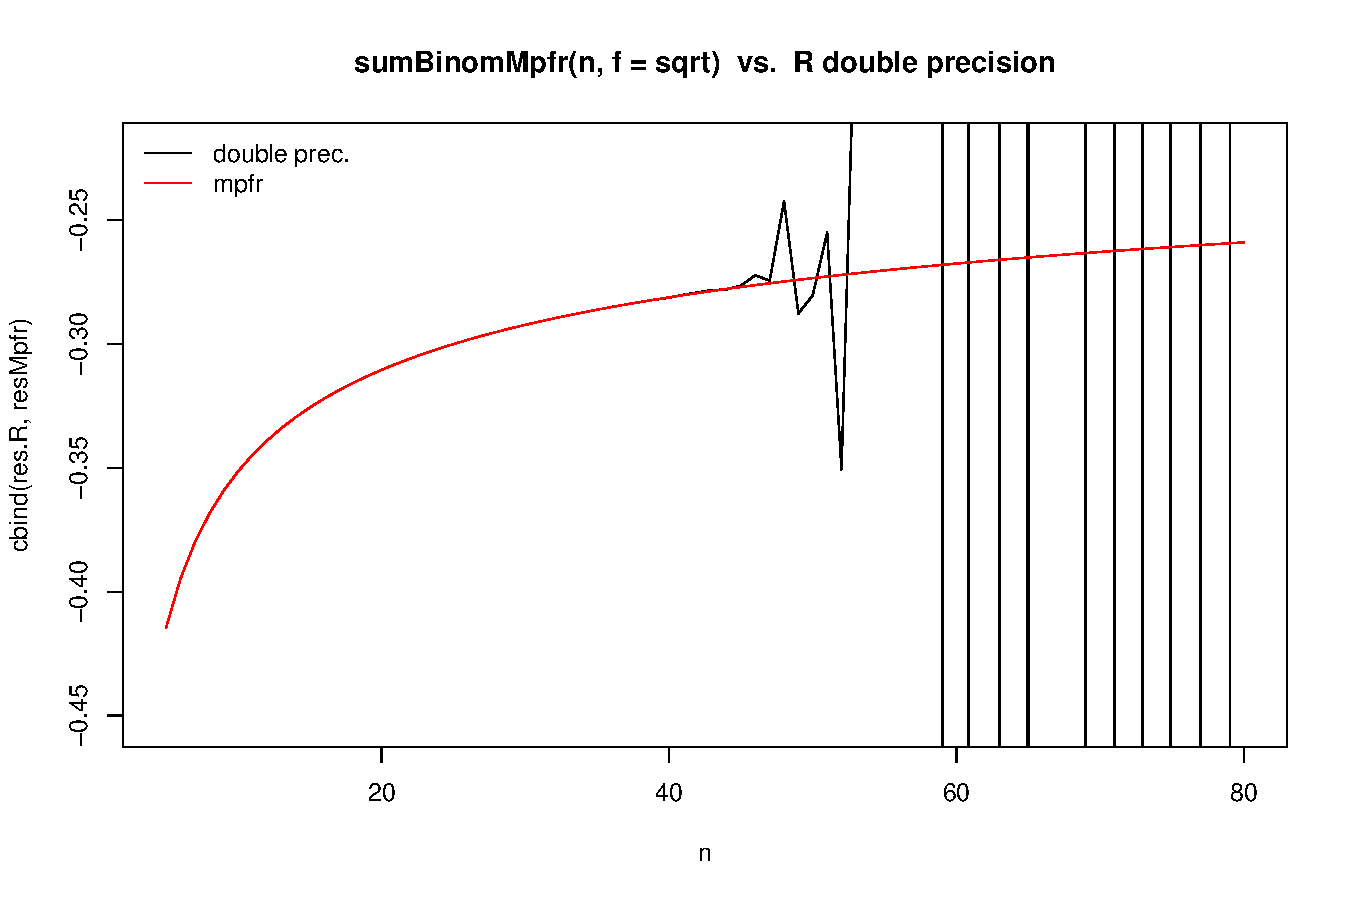
\includegraphics{sumBinC-sqrt-ex-2}
\end{frame}

%%% TeX-master: "Maechler_Rmpfr.tex"
